\section{Results}
\label{section:p450/results}
Both physical and fitted IDSite were able to achieve promising results predicting CYP2D6 sites of metabolism.
The physical model correctly identified 68 of 82 active sites of metabolism for a sensitivity of 0.829.
For inactive sites this model correctly identified 1054 of 1075 inactive sites with a specificity of 0.980.
The fit model performed similarly, and even slightly better, identifying 52 of 57 sites of metabolism (sensitivity of 0.912) in the training set and 25 of 25 in the test set (sensitivity of 1.0).
\begin{equation}
\mathrm{sensitivity} = \frac{TN}{TN + FP} = \frac{\text{\# of true sites of non-metabolism identified}}{\text{\#\ experimental\ sites\ of\ non-metabolism}}
\end{equation}

\begin{equation}
\mathrm{sensitivity} = \frac{TP}{TP + FN} = \frac{\text{\#\ of\ true\ sites\ of\ metabolism\ identified}}{\text{\#\ experimental\ sites\ of\ metabolism}}
\end{equation}

\begin{table}[h]
\singlespace
\footnotesize
\centering
\begin{tabular}{cccccccccc}
\hline
	&	&Physical	&	&	&Fitted	&	&	&	&\\
Compound \#	&Compound Name	&TP	&FP	&FN	&TP	&FP	&FN	&	&\\
\hline
1	&4-methoxyamphetamine	&1	&0	&0	&1	&0	&0	&	&\\
2	&Amitriptyline	&2	&2	&0	&2	&0	&0	&	&\\
3	&Aprindine	&4	&0	&1	&5	&0	&0	&	&\\
4	&Brofaromine	&1	&0	&0	&1	&0	&0	&	&\\
5	&Bufuralol	&0	&1	&1	&1	&0	&0	&	&\\
6	&Carvedilol	&1	&0	&2	&2	&0	&1	&	&\\
7	&Cinnarizine	&0	&2	&1	&0	&2	&1	&	&\\
8	&Clomipramine	&1	&0	&1	&1	&0	&1	&	&\\
9	&Codeine	&1	&0	&0	&1	&0	&0	&	&\\
10	&Desipramine	&2	&0	&0	&2	&0	&0	&	&\\
11	&Dextromethorphan	&1	&0	&0	&1	&0	&0	&	&\\
12	&Dihydrocodeine	&1	&1	&0	&1	&0	&0	&	&\\
13	&Ethylmorphine	&1	&0	&0	&1	&0	&0	&	&\\
14	&Flunarizine	&1	&0	&0	&1	&0	&0	&	&\\
15	&Fluperlapine	&1	&0	&0	&1	&0	&0	&	&\\
16	&Hydrocodone	&1	&0	&0	&1	&0	&0	&	&\\
17	&Imipramine	&2	&0	&0	&2	&0	&0	&	&\\
18	&Indoramine	&1	&0	&0	&1	&0	&0	&	&\\
19	&MDMA	&1	&0	&0	&1	&0	&0	&	&\\
20	&Methamphetamine	&1	&0	&0	&1	&2	&0	&	&\\
21	&Methoxyphenamine	&2	&0	&0	&2	&0	&0	&	&\\
22	&Metoprolol	&1	&0	&1	&2	&0	&0	&	&\\
23	&Mexiletine	&2	&0	&1	&2	&0	&1	&	&\\
24	&Mianserin	&1	&0	&0	&1	&0	&0	&	&\\
25	&Mirtazapine	&0	&1	&1	&1	&1	&0	&	&\\
26	&Nortriptyline	&1	&1	&0	&1	&0	&0	&	&\\
27	&Ondansetron	&2	&0	&0	&1	&0	&1	&	&\\
28	&Paroxetine	&1	&0	&0	&1	&0	&0	&	&\\
29	&Perhexiline	&2	&0	&0	&2	&0	&0	&	&\\
30	&Propafenone	&1	&1	&0	&1	&1	&0	&	&\\
31	&Propranolol	&2	&2	&0	&2	&1	&0	&	&\\
32	&Tamoxifen	&1	&0	&0	&1	&0	&0	&	&\\
33	&Terfenadine	&3	&0	&0	&3	&0	&0	&	&\\
34	&Tiracizine	&1	&2	&0	&1	&1	&0	&	&\\
35	&Tropisetron	&2	&0	&1	&3	&0	&0	&	&\\
36	&Venlafaxine	&1	&0	&0	&1	&0	&0	&	&\\
	&TOTAL	&47	&13	&10	&52	&8	&5	&	&\\
\hline
\end{tabular}
\caption{Results of physical and fitted IDSITE on training set of 36 compounds.}
\label{table:p450_training}
\end{table}

\begin{table}[h]
\singlespace
\footnotesize
\centering
\begin{tabular}{cccccccc}
\hline
 &  &  & Physical &  &  & Fitted & \\
Compound \# & Compound & TP & FP & FN & TP & FP & FN \\
\hline
37 & Atomoxetine & 0 & 1 & 1 & 1 & 2 & 0 \\
38 & Bicifadine & 1 & 2 & 0 & 1 & 0 & 0 \\
39 & Bupranolol & 1 & 0 & 0 & 1 & 0 & 0 \\
40 & Carteolol & 1 & 1 & 0 & 1 & 0 & 0 \\
41 & Chlorpromazine & 1 & 0 & 0 & 1 & 0 & 0 \\
42 & EMAMC & 1 & 0 & 0 & 1 & 0 & 0 \\
43 & Encainide & 1 & 1 & 0 & 1 & 1 & 0 \\
44 & Harmaline & 1 & 0 & 0 & 1 & 0 & 0 \\
45 & Harmine & 1 & 1 & 0 & 1 & 1 & 0 \\
46 & Ibogaine & 1 & 0 & 0 & 1 & 0 & 0 \\
47 & MAMC & 1 & 0 & 0 & 1 & 0 & 0 \\
48 & MMAMC & 1 & 0 & 0 & 1 & 0 & 0 \\
49 & MOPPP & 1 & 0 & 0 & 1 & 0 & 0 \\
50 & Oxycodone & 1 & 0 & 0 & 1 & 0 & 0 \\
51 & Spirosulfonamide & 2 & 0 & 0 & 2 & 0 & 0 \\
52 & Timolol & 2 & 0 & 2 & 4 & 0 & 0 \\
53 & Tolterodine & 0 & 1 & 1 & 1 & 1 & 0 \\
54 & Tramadol & 1 & 1 & 0 & 1 & 1 & 0 \\
55 & Tyramine & 2 & 0 & 0 & 2 & 0 & 0 \\
56 & Zotepine & 1 & 0 & 0 & 1 & 0 & 0 \\
 & Total & 21 & 8 & 4 & 25 & 6 & 0 \\
\hline
\end{tabular}
\caption{Results of physical and fitted IDSite on a test set of 20 compounds.
Note that for the physical model there is no training performed so results in the text are presented in a unified fashion for the training and test set.}
\label{table:p450_testing}
\end{table}






The fit model also correctly identified 709 of 717 inactive sites in the training set (specificity of 0.989) and 352 of 358 inactive sites in the test set (specificity of 0.983).
As the performance of the fit model is similar to that of the physical model, it does not appear that the fit model is over-parametrized to the training set.
Specific results for both models are presented in Tables \ref{table:p450_training} and \ref{table:p450_testing}, and the specific sites identified by both models as well as experiments are illustrated in Figures \ref{fig:idsite_traininga} and \ref{fig:idsite_test}. 

We believe that the parameters help account for some degree of noise in the molecular mechanics calculations.
The scaling of the binding energy difference, either to zero inside a window about the minimum energy pose, or by a factor of 0.58 decreases the relative weight of the molecular mechanics contribution relative the quantum contribution to the classifier.
This might imply that some sites are not being classified as active because they are not in the lowest energy conformation around the docked pose, suggesting that additional molecular mechanics sampling might further improve results.
However, as will be discussed later, the molecular mechanics stage already dominates the total time necessary for an IDSite prediction, and the current molecular mechanics procedure takes about 450 hours.

\begin{figure}[h!]
\centering
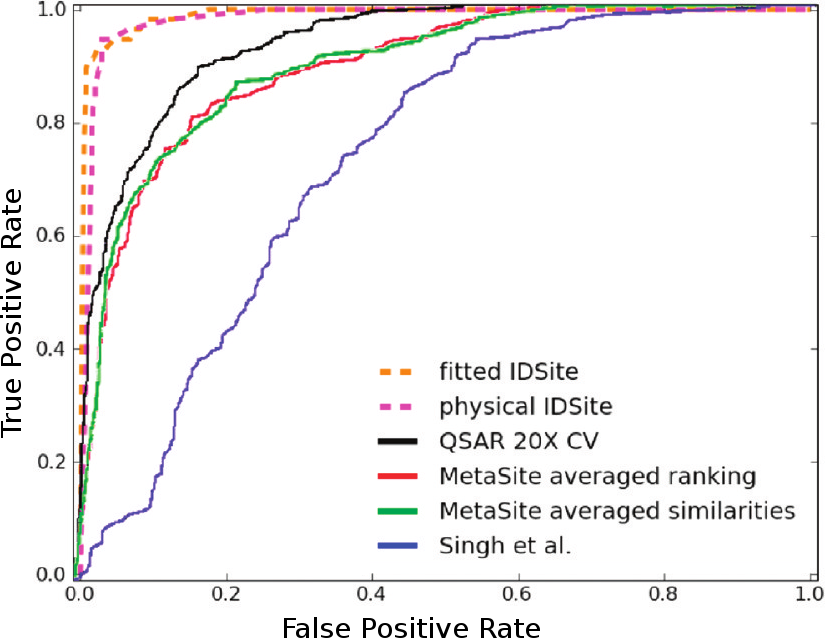
\includegraphics[width=0.5\textwidth]{figures/idsite/roc_other_methods.png}
\caption{A comparison of the performance of IDSite with a variety of other methods of predicting P450 sites of metabolism.
IDSite obtains the best performance, followed by a quantitative structure-activity relationship based method \protect\cite{sheridan2007empirical}.
Adapted from \protect\cite{sheridan2007empirical}.
}
\label{figure:idsite_other}
\end{figure}

\begin{figure}
\centering
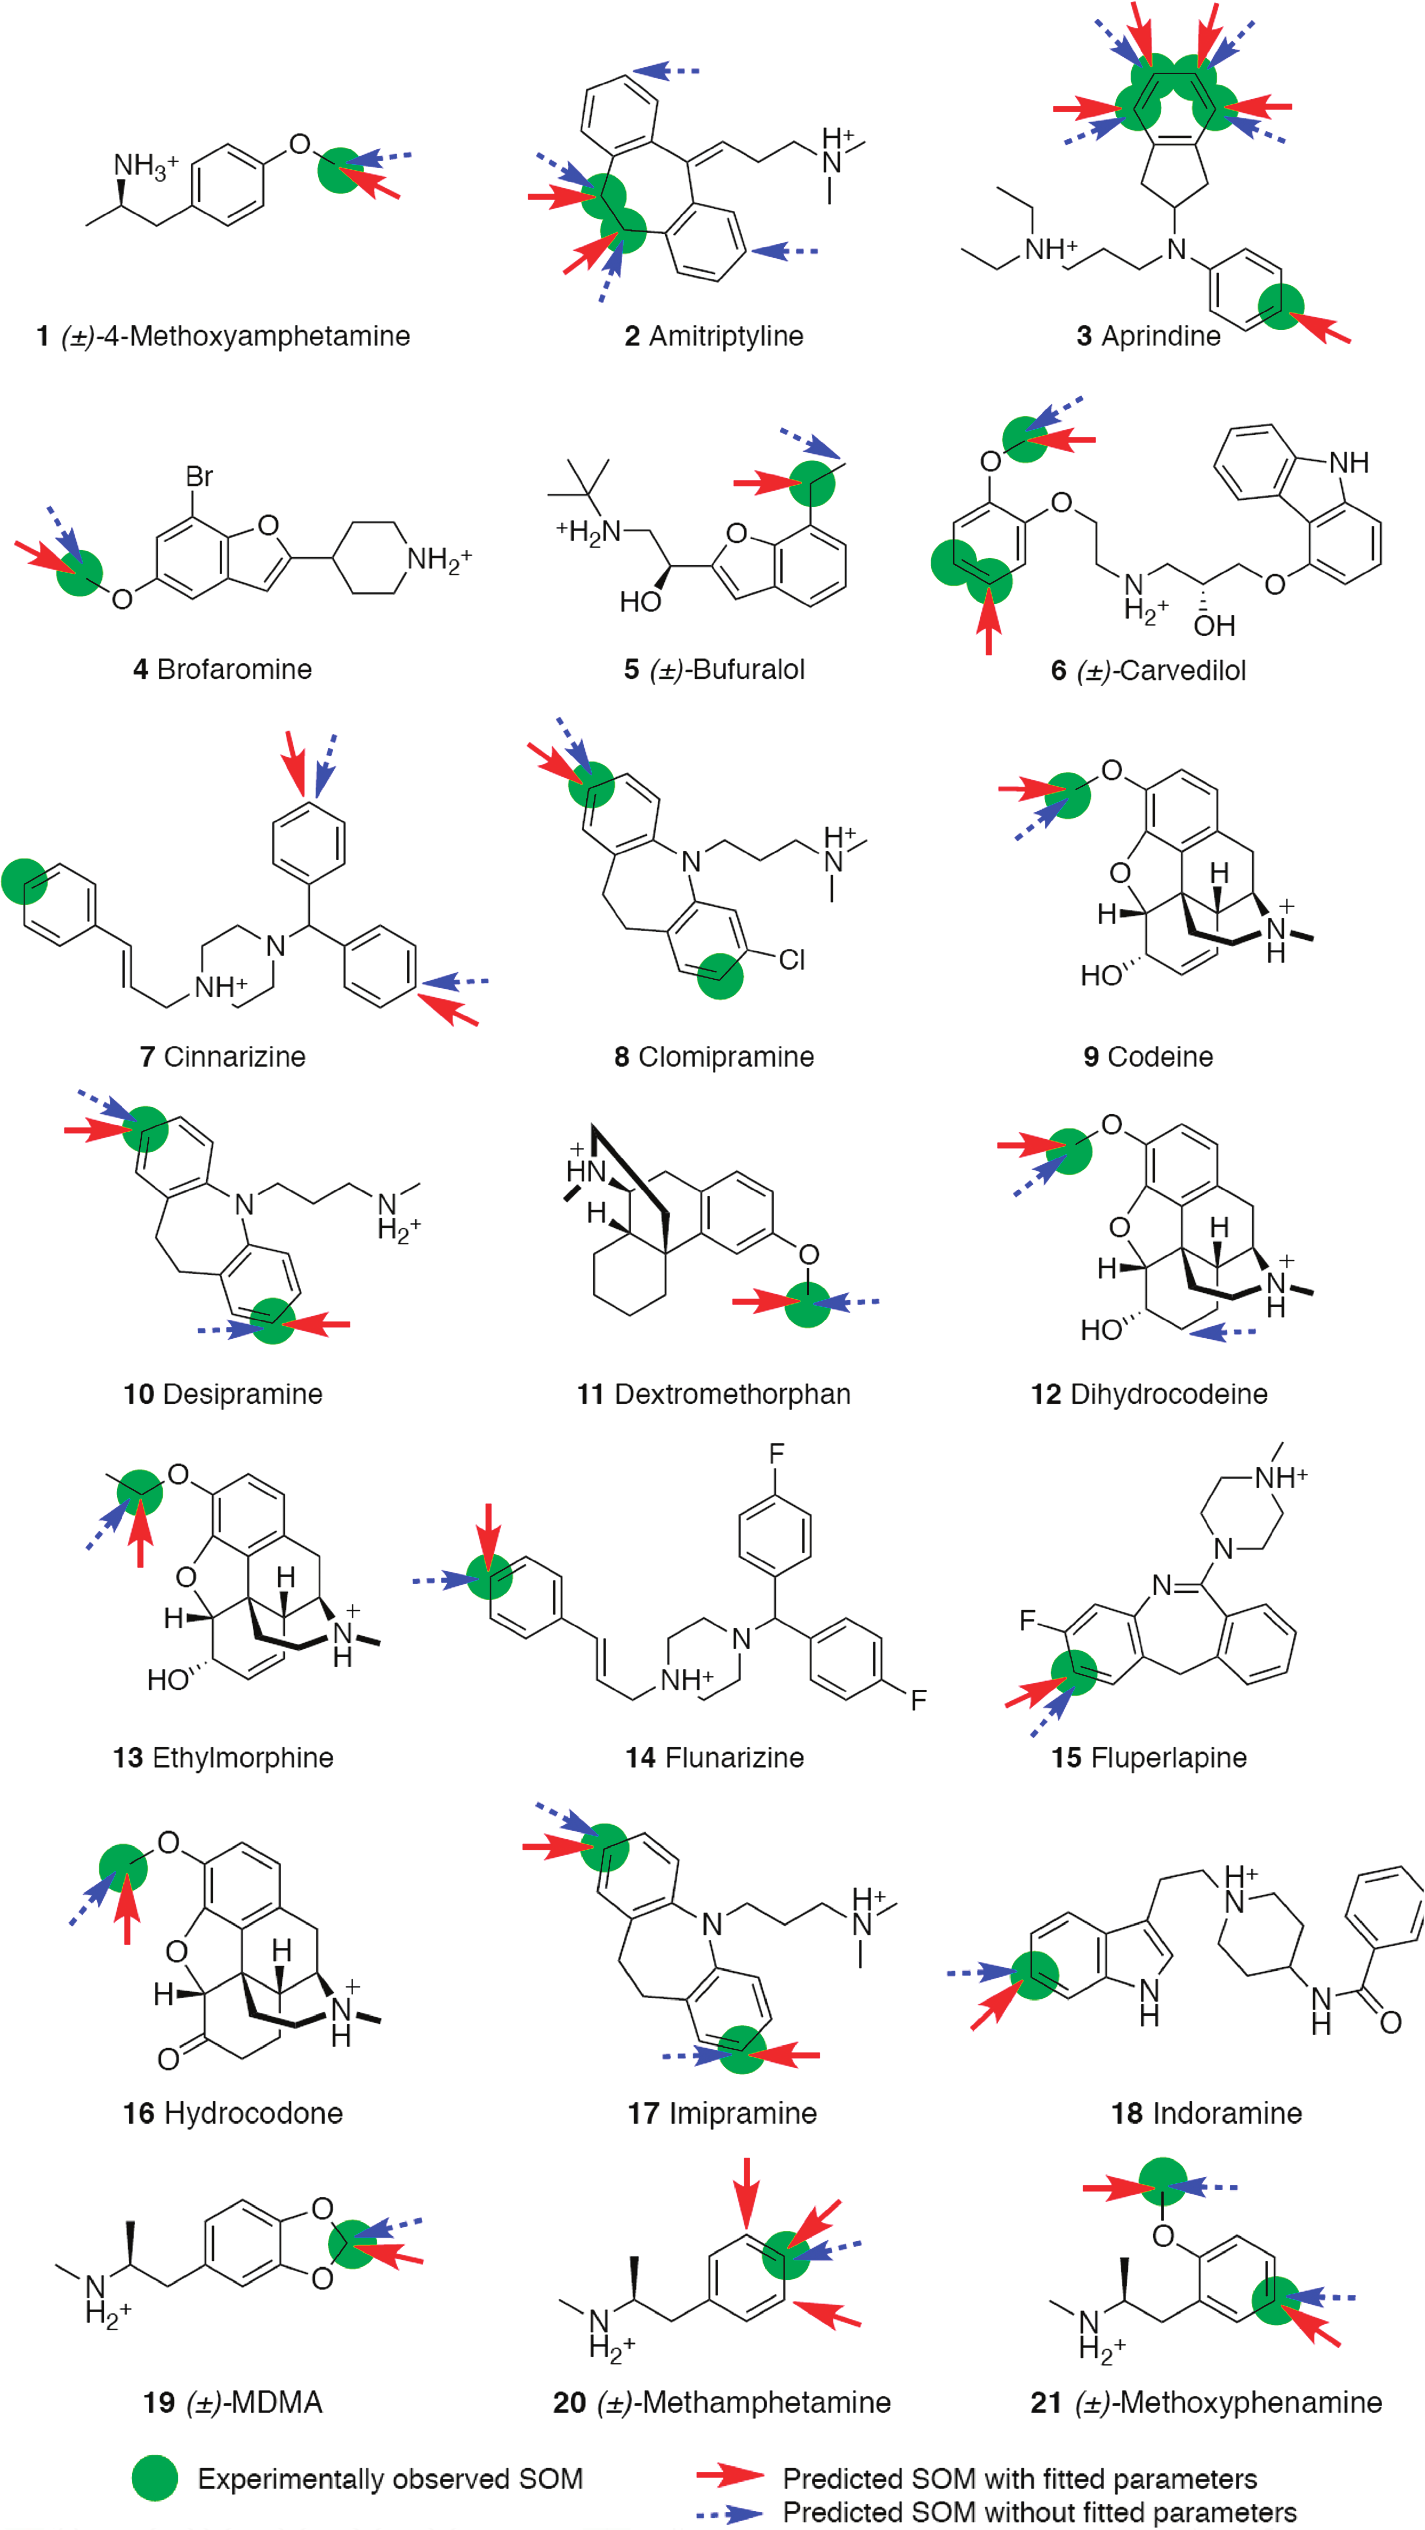
\includegraphics[width=0.65\textwidth]{figures/idsite/idsite_figure-007.png}
\caption{Physical and fitted IDSite predictions of sites of metabolism on the training set.}
\label{fig:idsite_traininga}
\end{figure}

\begin{figure}
\ContinuedFloat
\centering
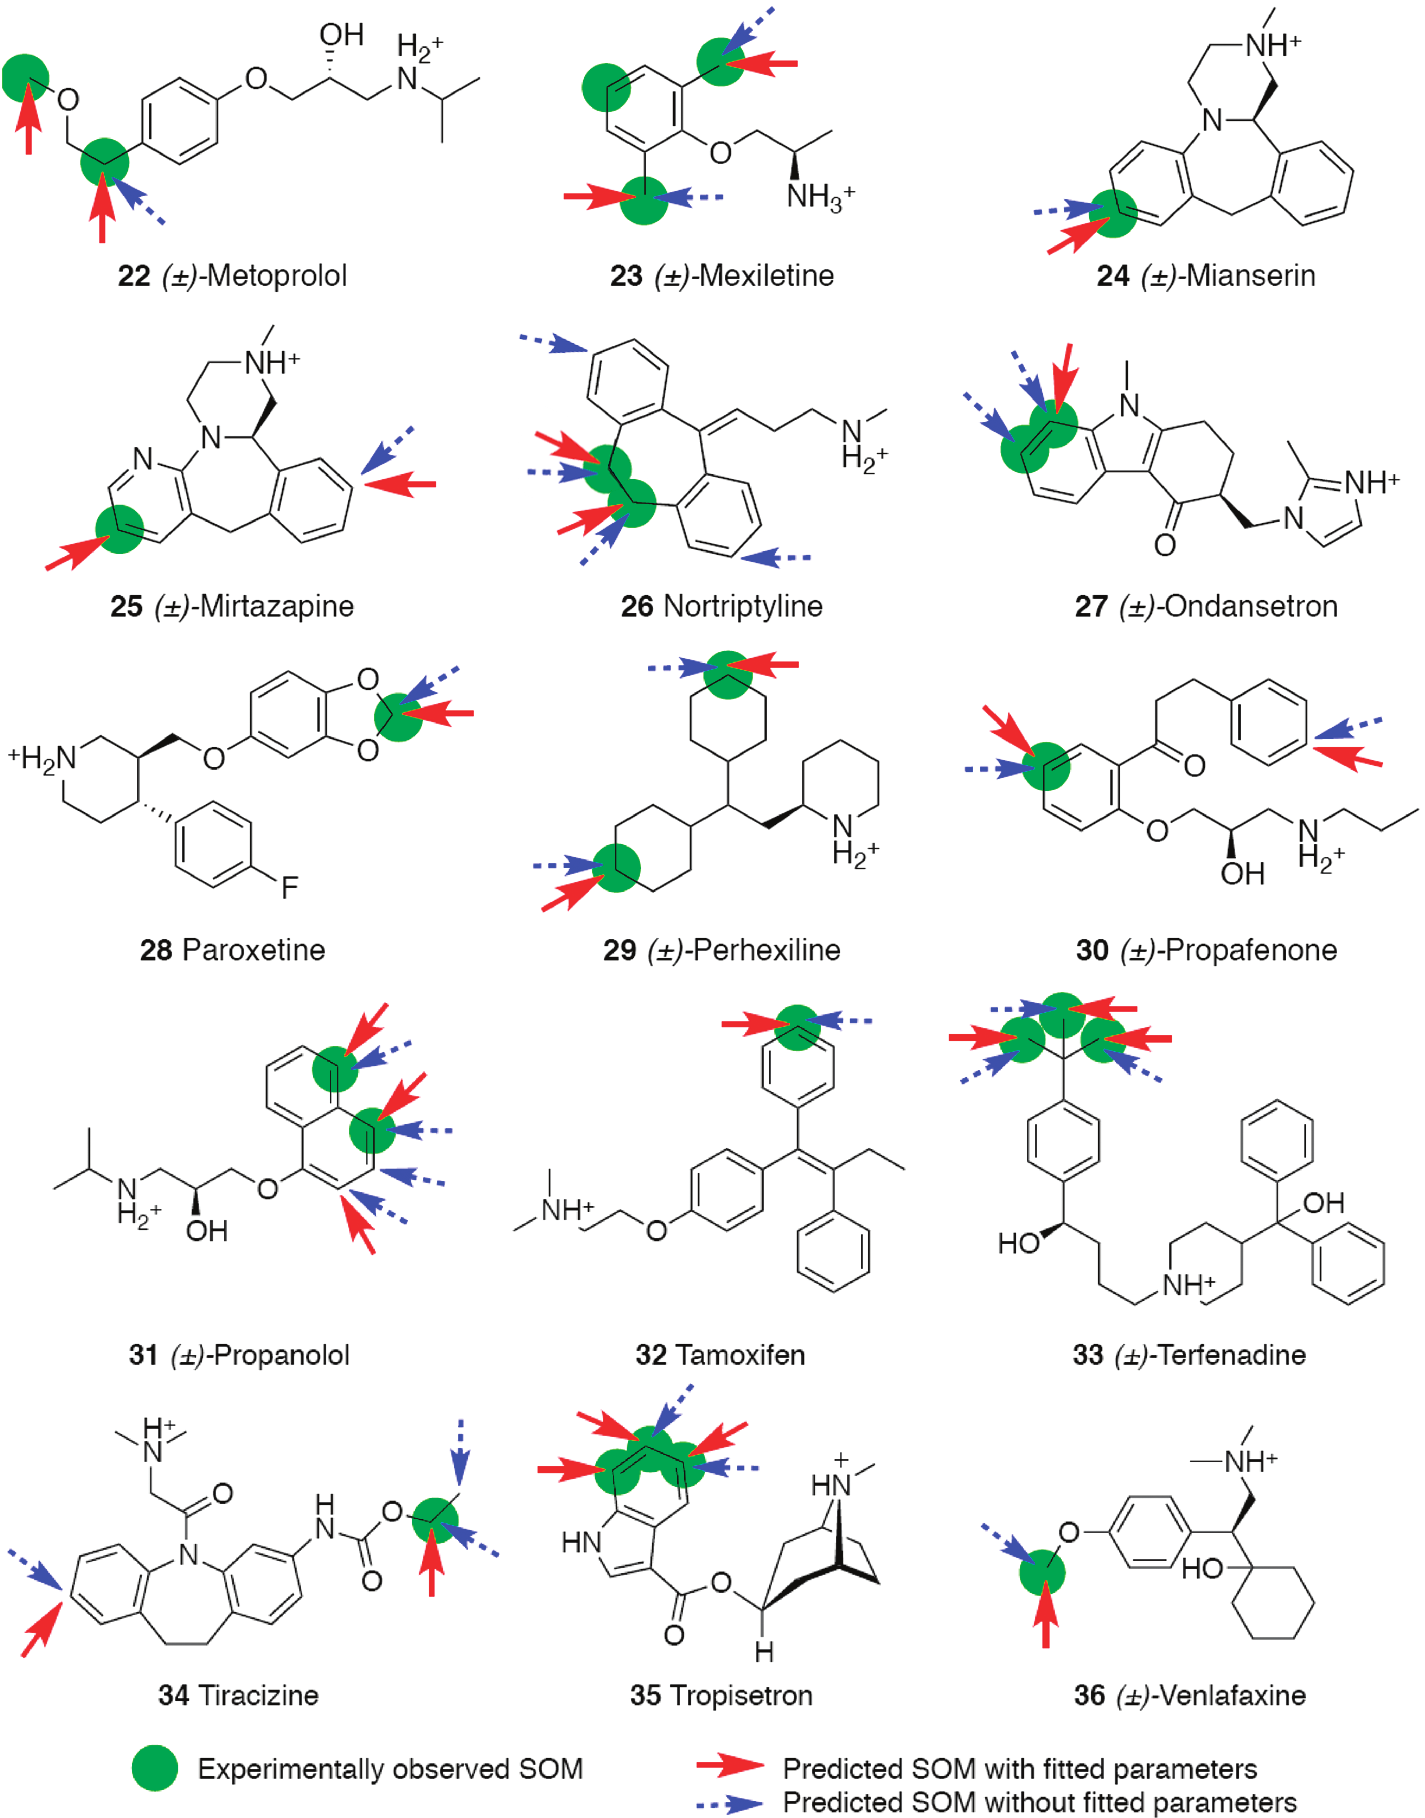
\includegraphics[width=0.65\textwidth]{figures/idsite/idsite_figure-008.png}
\caption{(continued)}
\label{fig:idsite_trainingb}
\end{figure}


\begin{figure}
\centering
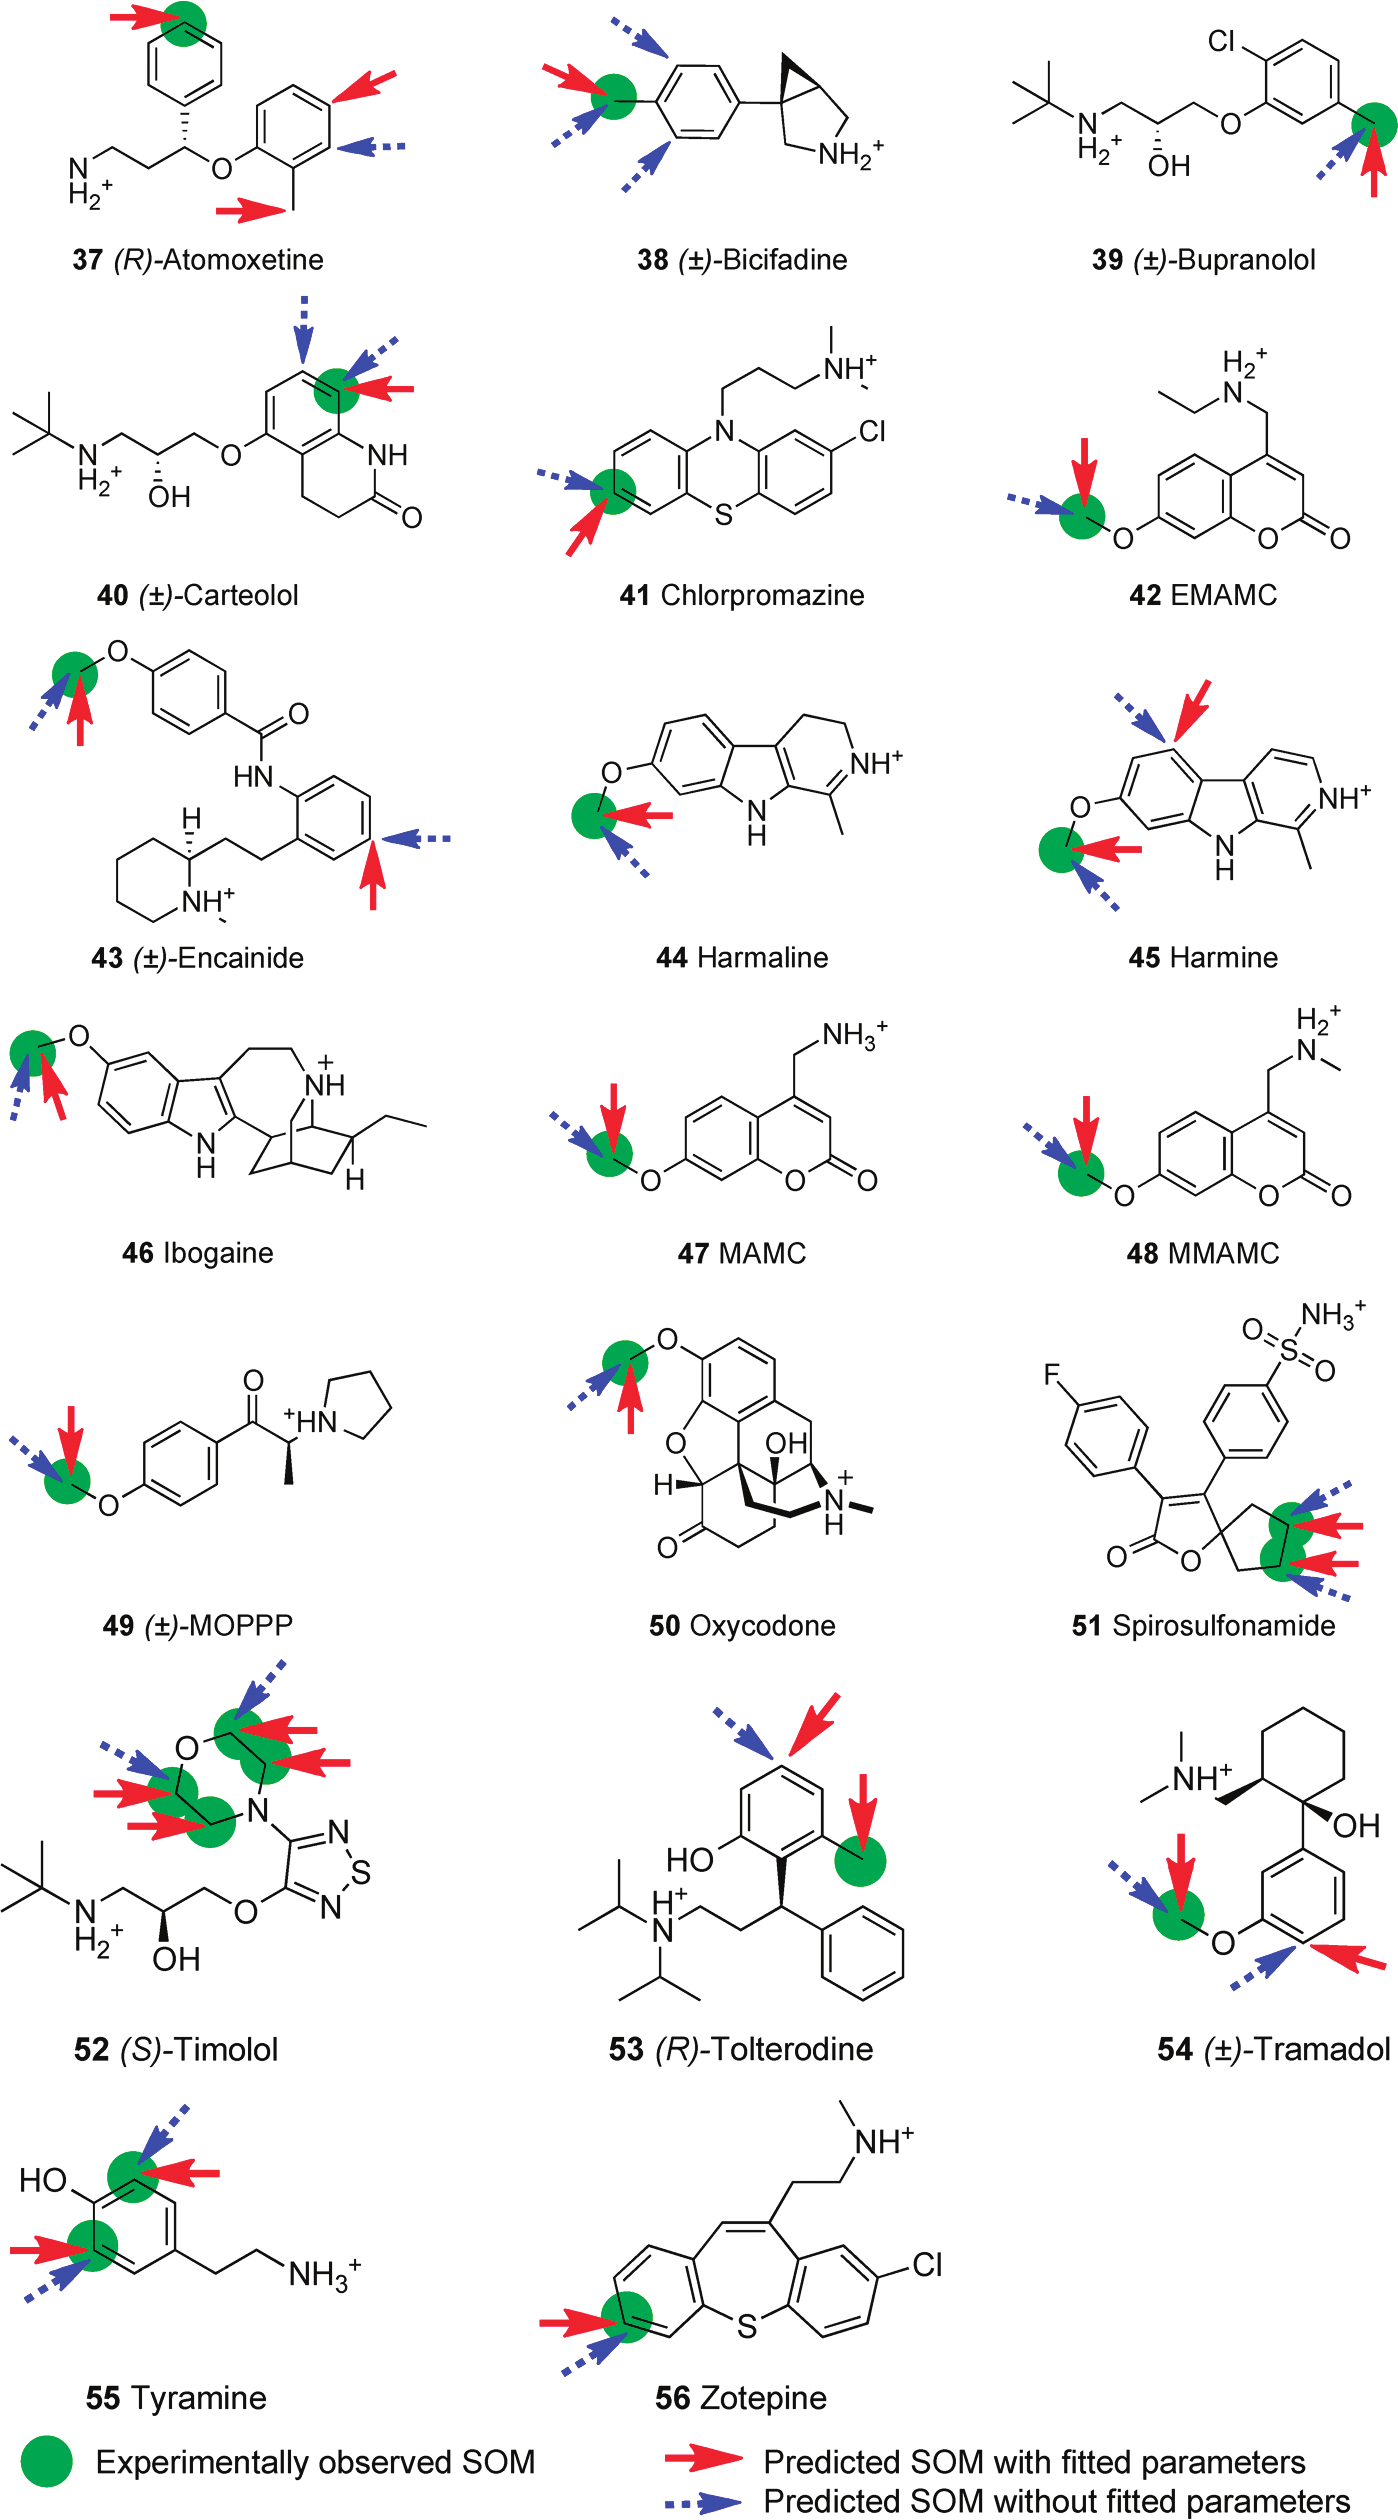
\includegraphics[width=0.65\textwidth]{figures/idsite/idsite_figure-009.png}
\caption{Physical and fitted IDSite predictions of sites of metabolism on the test set.}
\label{fig:idsite_test}
\end{figure}

